\documentclass[answers]{exam}
\usepackage{../../template}
\title{Assignment 7}
\author{Daniel Chua}
\begin{document}
\maketitle

\begin{questions}

\question{}

\begin{parts}

\part{Consider the case of a plasma being created at a constant rate $S$ [ion pairs/m$^3$/s] in a region between two infinite planes, separated by distance $L$. In the first moments of setting up the plasma, the electrons rush ahead to the walls, charging them negatively. Then in steady-state, an electric field exists in the plasma pulling the ions toward the wall and repelling the electrons. The electrons find themselves in a potential well (it’s minimum is at the midplane between the two walls). The electrons “dribble” over the top of the well to reach the walls at the same rate as the ions. The electron fluid is thus approximately static (its fluid velocity is very small compared to the electron sound speed) and therefore the electron density is related to the electric potential at each point in the plasma by the Boltzmann Relation. Write this relation.}

\begin{solution}
    $$n = n_0\exp\left(\frac{eV}{kT_e}\right)$$
\end{solution}

\part{Assume the ions move towards the wall in a one-dimensional, steady-state way subject to (i) their own pressure gradient force, (ii) the electric field, (iii) collisions with a stationary neutral gas background. $B = 0$. Write down the momentum conservation equation for the ions. Assume $Te = Ti$ and that both are constant in space.}

\begin{solution}
    $$\del{v_i}{t} + v_i\del{v_i}{x} = \frac{q}{m_i}E - \frac{kT}{m_in_i} \frac{dn_i}{dx} - \nu_{in} v_i - \frac{v_i}{n_i}S$$
\end{solution}

% b. assume momentum lost -m_i vS

\part{The conservation of ion mass equation is
$$\frac{d}{dx}(n_iv_i) = S$$
Use this with the momentum eqn. for the ions to find an expression for $\frac{dv_i}{dx}$ which shows that the plasma solution “blows up”, ie., $\frac{dv_i}{dx} \rightarrow \infty$ when $v_i$ reaches the ion acoustic sound speed: $c_s = \left(\frac{k(T_e + T_i)}{m_i}\right)^{1/2}$. (This singularity corresponds to the transition from the plasma to the sheath at the wall.)}

\begin{solution}
    Take $n_e = n_i = n$. Using the Boltzmann relation,
    \begin{align*}
        \frac{dn}{dx} &= \frac{ne}{kT_e} \frac{dV}{dx} \\
                      &= -E \frac{ne}{kT_e} \\
        E &= -\frac{kT_e}{ne} \frac{dn}{dx}
    \end{align*}
    Substituting,
    \begin{align*}
        \del{v_i}{t} + v_i\del{v_i}{x} &= -\frac{e}{m_i} \times \frac{kT_e}{ne} \frac{dn}{dx} - \frac{kT}{m_in} \frac{dn}{dx} - \nu_{in}v_i - \frac{v_i}{n} S \\
        \del{v_i}{x} &= -\frac{1}{v_i} \del{v_i}{t} - \frac{k(T_e+T_i)}{nm_iv_i} \frac{dn}{dx} - \nu_{in} - \frac{S}{n} \\
                     &= -\frac{1}{v_i} \del{v_i}{t} - \frac{c_s^2}{nv_i} \left(\frac{S}{v_i} - \frac{n}{v_i} \frac{dv_i}{dx}\right) - \nu_{in} - \frac{S}{n} \\
                     &= -\frac{1}{v_i} \del{v_i}{t} - \frac{S}{n} \left(1 + \frac{c_s^2}{v_i^2}\right) - \nu_{in} + \frac{c_s^2}{v_i^2} \frac{dv}{dx} \\
                     &= -\frac{v_i}{v_i^2-c_s^2} \del{v_i}{t} - \frac{S}{n} \left(\frac{v_i^2+c_s^2}{v_i^2-c_s^2}\right) - \frac{\nu_{in}v_i^2}{v_i^2-c_s^2}
    \end{align*}
    As $v_i$ reaches $c_s$, the denominators of the terms on the right go to zero, so $\del{v_i}{x}$ blows up.
\end{solution}
% c. n_e = n_i = n
    % use Boltzmann to find E = -dV/dx
    % P_i = nkT, dP/dx = kT dn/dx

\part{Find the generalization to the Boltzmann Relation in terms of the electron Mach number. Clearly at the edge of the plasma $v_e = v_i = c_s$. What then is the largest error in using the uncorrected Boltzmann Relation for the electrons assuming $T_e = T_i$?}

\begin{solution}
    Neglecting collisions and the source term, the momentum equation is
    \begin{align*}
        \del{v_e}{t} + v_e \del{v_e}{x} &= \frac{qE}{m_e} - \frac{1}{m_en_e} \frac{dP}{dx} \\
        c_e \del{M}{t} + c_e^2 M \del{M}{x} + \frac{eE}{m_e} &= -\frac{kT}{m_en_e} \frac{dn}{dx} \\
        -\frac{m_ec_edx}{kT} \left(\del{M}{t} + c_e M\del{M}{x}\right) + \frac{eE}{kT} dV &= \frac{dn}{n} \\
        -\frac{m_ec_e}{kT} \left(\frac{dx}{dt}dM + c_eMdM\right) + \frac{eE}{kT} dV &= \frac{dn}{n} \\
        -\frac{m_ec_e^2}{kT} \times 2MdM + \frac{eE}{kT} dV &= \frac{dn}{n} \\
        -16MdM + \frac{eE}{kT} dV &= \frac{dn}{n} \\
        n &= n_0\exp\left(\frac{eE}{kT} - 8M^2\right)
    \end{align*}
    The error is the extra exponential term, i.e. $\exp(8M^2)$. At $v_i = v_e = c_s$, the square of the Mach number is
    \begin{align*}
        M^2 &= \frac{c_s^2}{c_e^2} \\
            &= \frac{2kT}{m_i} \div \frac{8kT}{m_e} \\
            &= \frac{m_e}{4m_i}
    \end{align*}
    and the error becomes $\exp\left(\frac{2m_e}{m_i}\right) \approx 1.00109$. Then the percentage error is $0.109\%$, which is not too significant, considering how many approximations were made in the derivations.
\end{solution}
% d. neglect collisions in e mom eqn
    % neglect source term
    % get n = n_0 exp[eV(some fraction)]
    % use v_e^max = c_s to compare magnitude of terms
    % use continuity relation to relate velocity gradient to density gradient

\end{parts}

\question{The electron temperature and density in a conventional low pressure discharge tube such as a neon light or fluorescent tube. Example of H$^2$ as working gas.}

%% Q2 (there are 2 graphs in Dolan Fig 3C4, p54) (ignore factors of 2) (see last year's quiz)

\begin{parts}

\part{Show that the particle balance per unit length of tube leads to the following relation.}

\begin{solution}
    Production rate is equal to loss rate, so
    \begin{align*}
        Vn_en_g\langle \sigma v\rangle_{iz} &= \Gamma_e A \\
        \frac{r}{2}n_en_g \langle \sigma v \rangle_{iz} &= \frac{1}{2} n_e c_s \\
        \frac{d}{2} n_g \langle \sigma v \rangle_{iz} &= c_s \\
        n_gd &= \frac{2c_s}{\langle \sigma v \rangle_{iz}}
    \end{align*}
    Compared with the given equation, this is off by a factor of 2, which is fine according to Professor Davis.
    The curve is valid until
    \begin{align*}
        \lambda &= \frac{d}{2} \\
        \frac{1}{n_g\sigma_{in}} &= \frac{d}{2} \\
        \frac{2}{\sigma_{en}} &= n_gd
    \end{align*}
    \begin{center}
    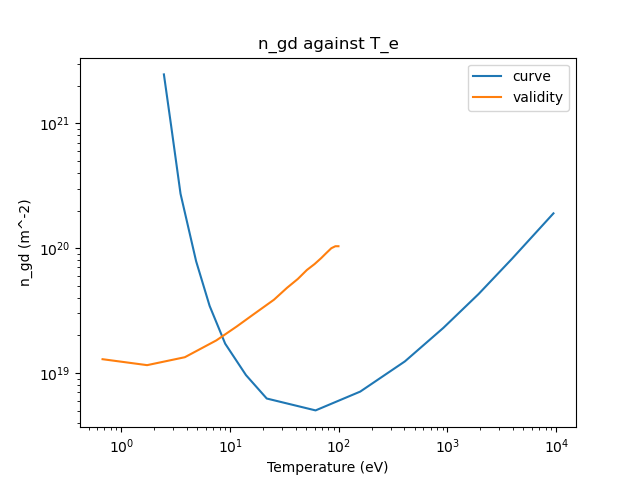
\includegraphics[scale=0.5]{q2a.png} \\
    \end{center}
    From the graph, equality is at $T_e = 8.6 \unit{eV}$. This means the orange curve accurately describes the relationtion between $T_e$ and $n_gd$ until it reaches the intersection. There is a minimum value of $n_gd$, since the graph was derived with the assumption that $T_e >> T_i$. This does not hold with $n_g$ is too small.
\end{solution}


% a. Particle balance: flow to wall = Γ * area = production rate
    % λ = 1/(n_g*σ_{in}), λ > d/2, so ions accelerate out without being stopped

\part{Find the electrical conductivity assuming only e–n collisions. Thus find the ohmic power input, $P_\Omega$ to the electrons in W/m$^3$. Show that $P_\Omega \propto 1/n_e$. Show that $P_{e,\text{loss}} \propto n_e$, and so by equating electron energy gain to loss. Show that $n_e \propto j$, the current density. Find $n_e$ for the specific example here. With this value of ne, or taking $n_e = 5 \times 10^{16} \unit{m^{-3}}$ show that in fact it was correct to neglect e–i collisions in calculating $P_\Omega$.}

\begin{solution}
    Use $T_e = 10\unit{eV}$. Electrical conductivity is given by
    \begin{align*}
        \sigma &= \frac{ne^2}{m_e\nu_e} \\
               &= \frac{ne^2}{m_e\sigma_{en}\overline{c_e}n_g}
    \end{align*}
    From Figure 3B2, $\sigma_{en} = 10^{-19}$ at $T_e = 10\unit{eV}$. Mean speed of electrons is
    \begin{align*}
        \overline c_e &= \sqrt{\frac{8kT_e}{\pi m_e}} \\
                      &= 2.12 \times 10^6
    \end{align*}
    Then
    $$\sigma = \frac{n_e e^2}{m_e\sigma_{en}\overline{c_e} n_g} = 2.66 \times 10^{-16}n_e$$
    Ohmic power is then
    \begin{align*}
        P_\Omega &= \frac{j^2}{\sigma} \\
                 &= \frac{16I^2}{d^4\pi^2\sigma} \\
                 &= \frac{6.78 \times 10^{22}}{n_e} \unit{W.m^{-3}}
    \end{align*}
    The ohmic power output is then inversely proportional to $n_e$. \\
    To find energy loss, we are given that $5kT_e$ is lost per electron. Rate of electron loss is flux density scaled by surface area. Then
    \begin{align*}
        P_e &= 5kT_e\Gamma_e A \\
            &= 5kT_e \times \frac{1}{4} n_e\overline c_e \pi dL \\
            &= 4.00 \times 10^{-13}Ln_e
    \end{align*}
    This is proportional to $n_e$. \\
    Equating ohmic power input and power loss,
    $$P_\Omega \propto \frac{j^2}{n_e} \propto P_e \propto n_e \Rightarrow j^2 \propto n_e^2 \Rightarrow n_e \propto j$$
    \begin{align*}
        \frac{\pi d^2L}{4} P_\Omega &= 4.00 \times 10^{-13}Ln_e \\
        4.79 \times 10^{19} &= 4.00 \times 10^{-13}n_e^2 \\
        n_e^2 &= 1.20 \times 10^{32} \\
        n_e &= 1.10 \times 10^{16}
    \end{align*}
    Finally, we attempt to justify why we ignored $\nu_{ei}$. Using $n_e = 5 \times 10^{16}$,
    \begin{align*}
        \frac{\nu_{ei}}{\nu_{en}} &= \frac{10^{-15}n_eT_e^{3/2}}{\sigma_{en}\overline{c_e}n_g} \\
                                  &= 4.72 \times 10^{-4}
    \end{align*}
    which is very small. Since e-i collisions are negligible compared to e-n collisions, it is okay to neglect the former.
\end{solution}
% b. Assume L > λ
    % Electrical conductivity: σ = ne^2/(m_e *m ν_e); ν_e = ν_{en} = σ_{en} overline{c_e} n_g
    % loss → convection to walls
    % P_e, loss = 5k T_e Γ_e * area (ignore T_i since it is small)
    % Energy balance P_Ω = P_e, loss
    % note that one is a volume process, the other is a surface process

\part{To show $T_e >> T_i, T_g$. Calculate the energy transfer rate from electrons to ions and neutrals for $n_e = 10^{16} \unit{m^{-3}}$ and $n_g = 5 \times 10^{20} \unit{m^{-3}}$, and by comparing these rates to $P_\Omega$ confirm that $T_e >> T_i, T_g$.}

\begin{solution}
    For e-n transfers, transfer time is
    \begin{align*}
        \tau^E &= \frac{1}{\nu^E} \\
             &= \frac{m_g}{m_e\nu^{\text{mom}}} \\
             &= \frac{m_g}{m_e\sigma_{en}\overline{c_e}n_g} \\
             &= 3.47 \times 10^{-5} \unit{s}
    \end{align*}
    Power transfer rate is then
    \begin{align*}
        P &= \frac{E}{\tau} \\
          &= \frac{m_e\left(\overline{c_e}\right)^2n_e}{2\tau} \\
          &= 587 \unit{W.m^{-3}}
    \end{align*}
    For electron ion transfers, transfer time is
    \begin{align*}
        \tau^E &= \frac{m_i}{m_e\nu^{\text{mom}}} \\
               &= \frac{m_i}{m_e\times10^{-15}nT_e^{-3/2}} \\
               &= 0.367 \unit{s}
    \end{align*}
    Similarly, power transfer rate is
    $$P = \frac{E}{\tau} = 0.02 \unit{W.m^{-3}}$$
    Using the given $n_e$, $P_\Omega = 6.78 \times 10^6 \unit{W.m{-3}}$, which is much greater than the other power losses. Therefore, there is not a lot of energy transfer from electrons, hence $T_e >> T_i,T_g$.
\end{solution}
% c. Energy transfer: τ^E_{en} ~ 1/ν^E_{en} ~ 1/(m_e/m_g)ν^{mom}_{en}
    % τ^E_{ei} ~ 1/(m_e/m_i)ν^{mom}_{ei}
    % Power transfer rate = Energy content of e / transfer time
    % compare with P_Ω
    % See 2022 Quiz 4

\part{Consider next the collisional regime where ions experience collisions with neutrals in distances less than $d$. The radial plasma flow is now ambipolar. Take $T_i = T_g = 500$ K, constant. Assuming $T_e >> T_i$, find the ambipolar diffusion coefficient as a function of $T_e$ and by equating particle loss rates radially to the ionization rate find a new relation for $T_e(n_gd)$. Plot on the same graph as collisionless case.}

\begin{solution}
    \begin{align*}
        D_A &= \frac{T_e}{T_i} D_i \\
            &= \frac{T_e}{T_i} \times \frac{kT_i}{m_i\nu_{in}} \\
            &= \frac{kT_e}{m_i\sigma_{in}\overline c_i n_g}
    \end{align*}
    Equating particle loss with ionization rate,
    \begin{align*}
        D_a \times \frac{n_e}{r} \pi dL &= n_en_g\langle \sigma v \rangle_{iz} \times \frac{\pi d^2}{4} L \\
        \frac{2kT_e}{m_i\sigma_{in}\overline{c_i}} &= n_g^2\langle \sigma v \rangle_{iz} \times \frac{d^2}{4} \\
        T_e &= \frac{m_i\sigma_{in}\overline{c_i}n_g^2\langle \sigma v \rangle_{iz}d^2}{8k}
    \end{align*}
    Mean speed is
    \begin{align*}
        \overline c_i &= \sqrt{\frac{8kT_i}{\pi m_i}} \\
                      &= 2292 \unit{m.s^{-1}}
    \end{align*}
    At 500 K, $\sigma_{en} \approx 10^{-19}$. Plugging in the constants,
    $$T_e = 3.78 \times 10^{-24}n_g^2d^2\langle \sigma v \rangle_{iz}$$
    where $T_e$ can be completely determined by $n_gd$. The plot is then as follows (see orange line)
    \begin{center}
        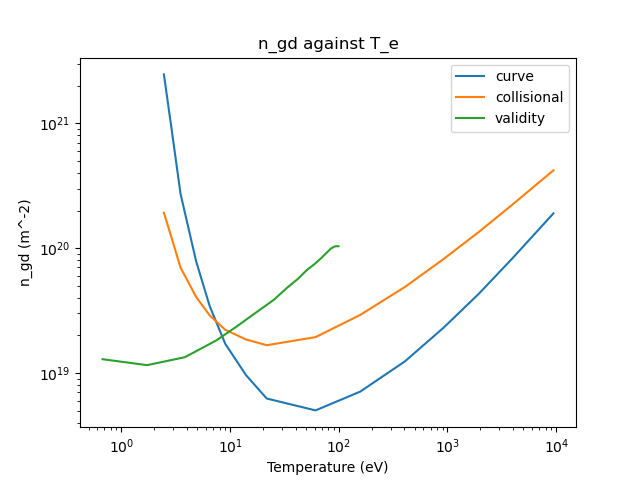
\includegraphics[scale=0.5]{q2d.png}
    \end{center}
\end{solution}
% d. Radial loss to walls Γ = D_A n/r 2 π rL
    % D_A ~ T_e/T_i D_i

\end{parts}

\question{Tokamak Safety Factor.}

\begin{solution}
    Recall
    $$B_p = \frac{\mu_0}{2\pi r} \int_0^r j(\rho)2\pi\rho d\rho$$
    For a uniform current profile,
    $$B_p = \frac{\mu_0}{2\pi r} \times j_0 \pi r^2 = \frac{\mu_0j_0r}{2}$$
    Substituting into $q$,
    \begin{align*}
        q &= \frac{B_Tr}{B_pR} \\
          &= \frac{2B_Tr}{\mu_0j_0rR} \\
          &= \frac{2B_T}{\mu_0j_0R}
    \end{align*}
    which has no $r$ dependence. For the more realistic profile,
    \begin{align*}
        B_p &= \frac{\mu_0}{2\pi r} \times \int_0^r j_0\exp\left(-\frac{3\rho^2}{a^2}\right) 2\pi\rho d\rho \\
            &= \frac{\mu_0j_0}{2r} \int_0^r \exp\left(-\frac{3\rho^2}{a^2}\right) d\left(\rho^2\right) \\
            &= \frac{\mu_0j_0}{2r} \frac{a^2}{3}\left(1 - \exp\left(-\frac{3r^2}{a^2}\right)\right)
    \end{align*}
    Then at $r = a$,
    \begin{align*}
        B_p &= \frac{\mu_0j_0a}{6} (1 - e^{-3}) \\
        q &= \frac{B_Tr}{B_pR} \\
          &= \frac{6B_Ta}{\mu_0j_0a(1-e^{-3})R} \\
          &\approx \frac{6B_T}{\mu_0j_0R}
    \end{align*}
    where we approximate $1 - e^{-3} \approx 1$. More care is needed for the $r = 0$ case. Since we cannot divide by 0, we write $q$ in terms of $r$ and take the limit as $r \rightarrow 0$.
    \begin{align*}
        q &= \frac{B_Tr}{B_pR} \\
          &= \frac{6B_Tr^2}{\mu_0j_0a^2\left(1-\exp\left(-\frac{3r^2}{a^2}\right)\right)R}
    \end{align*}
    As $r$ tends to 0, both the numerator and denominator tend to 0. Using L'H\^opital's rule,
    \begin{align*}
        q(r\rightarrow0) &= \lim_{r\rightarrow0} \frac{12B_Tr}{6\mu_0j_0rR} \\
                         &= \frac{2B_T}{\mu_0j_0R} \\
                         &\approx \frac{q(r=3)}{3}
    \end{align*}
\end{solution}

\question{}

\begin{parts}

    \part{A fully-ionized toroidal plasma, as in Fig. 5B2 of Dolan, is to have its current maintained by a gradually changing magnetic induction. It is desired to maintain a current of 20 MA approximately uniformly distributed over a plasma cross sectional area 30 $\unit{m^2}$ at $R$ = 10 m, with $T_e$ = 5 keV, $n = 5 \times 10^{20} \unit{m^{-3}}$. Estimate the plasma resistivity and required $dB/dt$ which must be provided in a transformer with core area 4 $\unit{m^2}$. (Hint: Use Ohm’s Law and Faraday’s Law.)}

\begin{solution}
    Using Ohm's Law,
    $$E = \frac{j}{\sigma} = \frac{I}{A\sigma} = \frac{20 \times 10^6}{30\sigma} = \frac{6.67 \times 10^5}{\sigma}$$
    Given the cross sectional area, the minor radius is found to be
    $$r = \sqrt{\frac{30}{\pi}}$$
    From Faraday's Law,
    \begin{align*}
        \nabla \times \vec E &= -\del{B}{t} \\
        \oint \nabla \times \vec E \cdot d\vec S &= \oint \frac{dB}{dt} dS \\
        \int \vec E \cdot d\vec l &= 4 \frac{dB}{dt} \\
        \frac{dB}{dt} &= \frac{1}{4} 2\pi RE \\
                      &= \frac{2\pi\times10}{4} \times \frac{6.67 \times 10^5}{\sigma} \\
                      &= \frac{1.05 \times 10^6}{\sigma}
    \end{align*}
    Now conductivity is
    \begin{align*}
        \sigma &= \frac{e^2n_e}{m_e\nu_{ei}} \\
               &= \frac{n_ee^2}{m_e10^{-15}n_eT^{-3/2}} \\
               &= \frac{e^2}{10^{-15}m_e\times5^{-3/2}} \\
               &= 3.14 \times 10^8
    \end{align*}
    Then resistivity is
    $$\rho = \frac{1}{\sigma} = 3.18 \times 10^{-9} \unit{\Omega.m}$$
    and
    $$\frac{dB}{dt} = 0.0333 \unit{T.s^{-1}} = 33.3 \unit{mT.s^{-1}}$$
\end{solution}

% a. Ohm's law E = j/σ
    % Faraday's Law ∇ × E = -∂B/∂t ⇒ integrate over surface
    % Dolan p 103 - 105

\begin{solution}
    For the primary circuit, $B \propto NI$. For there to be a constant $\frac{dB}{dt}$, $I$ needs to grow linearly. It would not help to have two of them, since that is simply superposition. You would get the same result by putting the 2 power supplies in series. Inductors are governed by
    $$v = L \frac{dI}{dt}$$
    Current needs to increase to maintain a voltage, but there are obviously numerous restrictions on maximum current (e.g. power consumption). Hence a given voltage can only be maintained for so much time until this limit is hit. Therefore, it only makes sense to characterize power supply by voltage seconds. A higher voltage can be reached with the trade-off of less time, since current takes less time to reach its maximum. In fact,
    $$Vt = L \frac{dI}{dt}t \approx LI$$
    where $I$ is the maximum current.
\end{solution}
% b. Primary circuit B ∝ NI
    % Inductor V = L dI/dt
    % Iron saturations at 2T, so that's no good, we use air

\end{parts}
%% Q5
% www.tokamak.info

\question{}

\begin{parts}

\part{Evaluate the Greenwald density limit for C-mod, JT-60U and ASDEX-Upgrade.}

\begin{solution}
    The Greenwald density limit is given by
    $$\overline n_e \leq n_G = \frac{I}{\pi a^2} \times 10^{20}$$
    where $I$ has units of MA and $a$ has units of metres. \\
    For C-mod, $I = 2, a = 0.22$, so the density limit is $n_G = 1.32 \times 10^{21} \unit{m^{-3}}$. For JT-60U, $I = 1.4, a = 0.5-0.8$. Taking the "average" value of $a^2$, i.e.
    $$E(a^2) = \frac{1}{0.3} \int_{0.5}^{0.8} x^2dx = 0.43$$
    which gives $n_G = 1.04 \times 10^{20} \unit{m^{-3}}$. Finally, for the ASDEX-Upgrade, $I = 5, a = 1.0$, so $n_G = 1.59 \times 10^{20} \unit{m^{-3}}$.
\end{solution}

\part{Using the L-mode empirical scaling for $\tau_E$ , estimate the maximum possible Lawson parameter for these 3 tokamaks. Additional input power will improve both $n_G$ and $\tau_E$.}

\begin{solution}
    The maximum Lawson parameter is given by $n_G\tau_E$, where the former is calculated above, and the latter is given by
    $$\tau_L = 0.048 \frac{I^{0.85}R_0^{1.2}a^{0.3}\kappa^{0.5}\overline{n}^{0.1} B_0^{0.2}A^{0.5}}{P^{0.5}}$$
\end{solution}
\end{parts}

\end{questions}
\end{document}
